\documentclass{standalone}
\usepackage{tikz}

\begin{document}
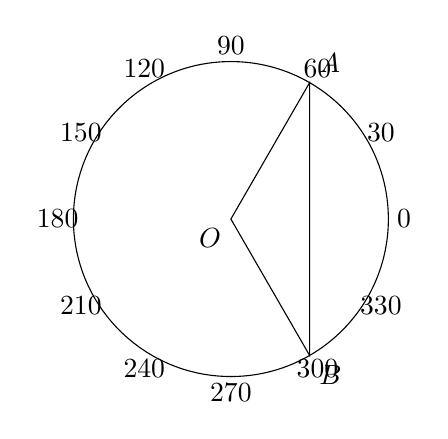
\begin{tikzpicture}[scale=2]
    % Draw the unit circle
    \draw (0,0) circle (1);
    
    % Draw the triangle
    \draw[fill=white] (0,0) -- (60:1) -- (300:1) -- cycle;
    
    % Label the circle
    \foreach \angle in {0, 30, ..., 330} {
        \draw (\angle:1.1) node {\angle};
    }
    
    % Label the triangle vertices
    \draw (60:1) node [above right] {$A$};
    \draw (300:1) node [below right] {$B$};
    \draw (0,0) node [below left] {$O$};
\end{tikzpicture}
\end{document}